\documentclass{beamer}
%\usecolortheme[named=green]{structure}
\mode<presentation> {
\usetheme{Copenhagen} % Pretty neat, soft color.
%\setbeamertemplate{footline}[page number]
\setbeamercovered{transparent}
\setbeamercovered{invisible}
% To remove the navigation symbols from the bottom of slides%
\setbeamertemplate{navigation symbols}{} 
}
\usepackage{graphicx}
\usepackage{bm} 
\usepackage{wasysym}
\title[ECML/PKDD 2011 demo session (demo \#10)]{InFeRno - an Intelligent Framework for Recognizing Pornographic Web pages}
\author{\bf{\underline{S. Karavarsamis}, N. Ntarmos and K. Blekas }}
\institute[UoI]
{
Department of Computer Science\\
University of Ioannina, Greeece \\
\medskip
{\{cs061205, ntarmos, kblekas\}@cs.uoi.gr}
}
\date{\today}
\begin{document}
\begin{frame}
\titlepage
\end{frame}
\begin{frame}
\frametitle{Problem preliminaries and intuition}
\begin{block}
{}
Given the unstructured and chaotic nature of the Web, we seek statistical mining techniques to assimilate detection of pornographic content by exploiting visual semantics of imagery (images, video, etc).
\end{block}
\emph{Some driving goals out of this demo:}
\begin{enumerate}
\item measure contribution of feature-based visual classification techniques alone for web page content assessment via a transparent-proxying and a content adaptation testbed (ICAP)
\item introduce "bikini" class to enhance accuracy of nudity-score estimation and/or cope with tolerance in presence of minuscule nude-like images (e.g. bikini) in benign web pages
\item evaluate discriminative performance of a diverse set of computationally-friendly low-level visual features in a real-time multi-class SVM classification scheme
\end{enumerate}
\end{frame}

\begin{frame}
\frametitle{InFeRno architecture}
\begin{center}
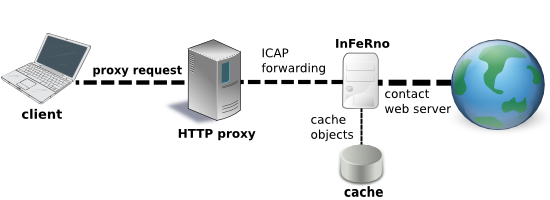
\includegraphics[scale=0.6]{images/network_diagram.png}
\begin{enumerate}
\item A systems administrator can tweak network parameters and adapt nudity acceptance thresholds to an orginization's needs
\item Zero-knowledge implementation of customized filtering directives within InFeRno
\item InFeRno's implemented as an ICAP module decoupled from the classification and caching processes
\item Implementation of a fast ISAM-based cache for fast web object I/O (lookups, updates, etc)
\end{enumerate}
\end{center}
\end{frame}

\begin{frame}
\frametitle{InFeRno vs POESIA}
\begin{enumerate}
\item Performance on image classification was evaluated and compared to that of POESIA in terms of CPU time consumption (see figure below).
\item The generalization performance of the InFeRno one-against-all SVM classification scheme was comparable to that of POESIA.
\end{enumerate}
\begin{block}
{}
A 4x speedup was observed on our manually collected dataset (660 nude images, 600 bikini images and 4500 benign images).
\end{block}
\begin{center}
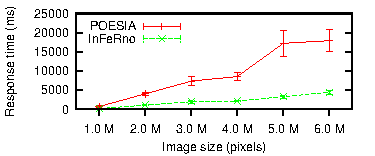
\includegraphics[scale=1.3]{images/scatter-p-t-all-bars.pdf}
\end{center}
\end{frame}

\begin{frame}
\centerline{For more information, please feel free to stop by our demonstration desk!}
\centerline{\bf{Thank you for your attention! \smiley}}
\end{frame}
\end{document} 
